\documentclass[10pt]{beamer}
\usetheme{metropolis}

% ── Packages ──
\usepackage{amsmath,amssymb,amsthm}
\usepackage{tikz}
\usetikzlibrary{positioning,arrows.meta,calc}
\usepackage{graphicx}
\usepackage{array}
\usepackage{etoolbox}

% ── Theorem environments ──
\theoremstyle{definition}
\newtheorem{defi}{Definition}[section]
\newtheorem{prop}{Proposition}[section]
\newtheorem{thm}{Theorem}[section]

% Custom theorem styles with colors
\setbeamercolor{block title}{bg=red!75!black,fg=white}
\setbeamercolor{block body}{bg=yellow!10!white}

\AtBeginEnvironment{prop}{%
  \setbeamercolor{block title}{bg=yellow!75!black,fg=black}%
  \setbeamercolor{block body}{bg=yellow!10!white}%
}
\AtEndEnvironment{prop}{%
  \setbeamercolor{block title}{bg=red!75!black,fg=white}%
}

\AtBeginEnvironment{thm}{%
  \setbeamercolor{block title}{bg=yellow!75!black,fg=black}%
  \setbeamercolor{block body}{bg=yellow!10!white}%
}
\AtEndEnvironment{thm}{%
  \setbeamercolor{block title}{bg=red!75!black,fg=white}%
}

% ── Highlighting ──
\newcommand{\x}[1]{\alert{\textbf{#1}}}
\newcommand{\rd}[1]{{\color{red!70!black}#1}}
\newcommand{\bl}[1]{{\color{blue!70!black}#1}}
\newcommand{\gn}[1]{{\color{green!60!black}#1}}
\newcommand{\ora}[1]{{\color{orange!80!black}#1}}
\newcommand{\gry}[1]{{\color{gray}#1}}
\newcommand{\oplusperp}{\mathbin{\overset{\perp}{\oplus}}}
\newcommand{\Vcols}{\begin{pmatrix}|&|& &|\\ \bl{v_1}&\rd{v_2}&\cdots&\gry{v_n}\\ |&|& &|\end{pmatrix}}
\newcommand{\Ucols}{\begin{pmatrix}|&|& &|\\ \bl{u_1}&\rd{u_2}&\cdots&\gry{u_m}\\ |&|& &|\end{pmatrix}}
\newcommand{\Vrows}{\begin{pmatrix}-&\bl{v_1^T}&-\\ -&\rd{v_2^T}&-\\ &\vdots&\\ -&\gry{v_n^T}&-\end{pmatrix}}
\newcommand{\Urows}{\begin{pmatrix}-&\bl{u_1^T}&-\\ -&\rd{u_2^T}&-\\ &\vdots&\\ -&\gry{u_m^T}&-\end{pmatrix}}
\newcommand{\Sigdisplay}{\begin{pmatrix}\bl{\sigma_1}&0&\cdots&0\\ 0&\rd{\sigma_2}&\cdots&0\\ \vdots&\vdots&\ddots&\vdots\\ 0&0&\cdots&\gry{0}\end{pmatrix}}
\newcommand{\SigTsigdisplay}{\begin{pmatrix}\bl{\sigma_1^2}&0&\cdots&0\\ 0&\rd{\sigma_2^2}&\cdots&0\\ \vdots&\vdots&\ddots&\vdots\\ 0&0&\cdots&\gry{0}\end{pmatrix}}
\newcommand{\svdproduct}{\underbrace{\Ucols}_{U}\underbrace{\Sigdisplay}_{\Sigma}\underbrace{\Vrows}_{V^T}}

\title{Lecture 20: Singular Value Decomposition}
\subtitle{Balls, Gaussian Clouds, and Real Orthogonal Axes}
\date{}
\titlegraphic{}

\begin{document}
\begin{frame}[plain,shrink=10]
\titlepage
\end{frame}

% ═══════════════════════════════════════
% §1 MOTIVATION
% ADR: The opening must be visual and concrete. Start with the three-step
% picture (circle -> circle -> ellipse -> rotated ellipse), then state the
% algebraic goal A=U Sigma V^T. Avoid probability/covariance at the entrance.
% ═══════════════════════════════════════
\section{The Visual Question}

\begin{frame}{Today's Question}

$$
\underbrace{x\in\mathbb R^n}_{\text{input vector}}
\qquad
\xrightarrow{\quad
\underbrace{A}_{m\times n\text{ real matrix}}
\quad}
\qquad
\underbrace{Ax\in\mathbb R^m}_{\text{output vector}}.
$$

\vfill

Instead of asking for eigenvectors of $A$, ask a geometric question:

\vfill

\begin{center}
{\Large\x{What does $A$ do to the round unit ball?}}
\end{center}

\vfill

\begin{center}
\x{SVD is the axis system of that transformed shape.}
\end{center}

\end{frame}


\begin{frame}[fragile]{The Picture First: Circle to Ellipse}

\begin{center}
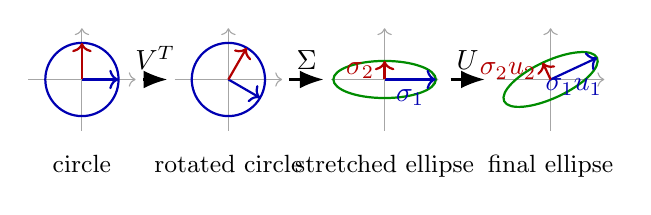
\begin{tikzpicture}[scale=0.62]
  \foreach \x/\label in {0/{circle},3.0/{rotated circle},6.2/{stretched ellipse},9.6/{final ellipse}} {
    \draw[->,gray!70] (\x-1.1,0) -- (\x+1.1,0);
    \draw[->,gray!70] (\x,-1.05) -- (\x,1.05);
    \node[below,font=\small] at (\x,-1.35) {\label};
  }

  \draw[blue!70!black,thick] (0,0) circle (0.75);
  \draw[blue!70!black,->,thick] (0,0)--(0.75,0);
  \draw[red!70!black,->,thick] (0,0)--(0,0.75);

  \begin{scope}[shift={(3.0,0)},rotate=-30]
    \draw[blue!70!black,thick] (0,0) circle (0.75);
    \draw[blue!70!black,->,thick] (0,0)--(0.75,0);
    \draw[red!70!black,->,thick] (0,0)--(0,0.75);
  \end{scope}

  \begin{scope}[shift={(6.2,0)}]
    \draw[green!55!black,thick] (0,0) ellipse (1.05 and 0.38);
    \draw[blue!70!black,->,thick] (0,0)--(1.05,0) node[midway,below] {$\sigma_1$};
    \draw[red!70!black,->,thick] (0,0)--(0,0.38) node[midway,left] {$\sigma_2$};
  \end{scope}

  \begin{scope}[shift={(9.6,0)},rotate=25]
    \draw[green!55!black,thick] (0,0) ellipse (1.05 and 0.38);
    \draw[blue!70!black,->,thick] (0,0)--(1.05,0) node[midway,below] {$\sigma_1u_1$};
    \draw[red!70!black,->,thick] (0,0)--(0,0.38) node[midway,left] {$\sigma_2u_2$};
  \end{scope}

  \draw[-{Latex[length=3mm]},thick] (1.25,0) -- node[above] {$V^T$} (1.75,0);
  \draw[-{Latex[length=3mm]},thick] (4.25,0) -- node[above] {$\Sigma$} (4.95,0);
  \draw[-{Latex[length=3mm]},thick] (7.55,0) -- node[above] {$U$} (8.25,0);
\end{tikzpicture}
\end{center}

\vspace{0.2cm}

\begin{center}
\x{The formula is visual: circle $\to$ circle $\to$ ellipse $\to$ rotated ellipse.}
\end{center}

\end{frame}


\begin{frame}[shrink=12]{Our Goal After the Picture}

\[
\scriptsize
\boxed{
A=
\underbrace{\Ucols}_{\substack{U\\\text{final output axes}}}
\underbrace{\Sigdisplay}_{\substack{\Sigma\\\text{axis lengths}}}
\underbrace{\Vrows}_{\substack{V^T\\\text{special input coordinates}}}
}.
\]

\vfill

\begin{center}
\x{The picture says: rotate to special coordinates, stretch, rotate back.}
\end{center}

\end{frame}


\begin{frame}[shrink=12]{The Three Actions}

\[
\scriptsize
A=
\underbrace{\Ucols}_{\substack{U\\\text{rotate again}}}
\underbrace{\Sigdisplay}_{\substack{\Sigma\\\text{stretch}}}
\underbrace{\Vrows}_{\substack{V^T\\\text{rotate}}}.
\]

\vfill

\begin{center}
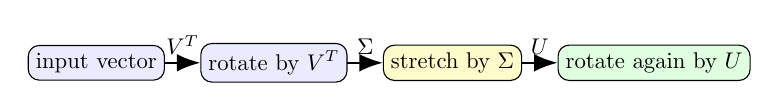
\begin{tikzpicture}[node distance=0.55cm,scale=0.82,transform shape]
  \node (x) [draw,rounded corners,fill=blue!8] {input vector};
  \node (coord) [draw,rounded corners,fill=blue!8,right=of x] {rotate by $V^T$};
  \node (stretch) [draw,rounded corners,fill=yellow!20,right=of coord] {stretch by $\Sigma$};
  \node (out) [draw,rounded corners,fill=green!12,right=of stretch] {rotate again by $U$};

  \draw[-{Latex[length=3mm]},thick] (x) -- node[above] {$V^T$} (coord);
  \draw[-{Latex[length=3mm]},thick] (coord) -- node[above] {$\Sigma$} (stretch);
  \draw[-{Latex[length=3mm]},thick] (stretch) -- node[above] {$U$} (out);
\end{tikzpicture}
\end{center}

\vspace{0.25cm}

\begin{center}
\x{Rotate, stretch, rotate again.}
\end{center}

\end{frame}

% ═══════════════════════════════════════
% §3 WHY A^T A
% ADR: Keep the reason for A^T A algebraic and short. Start from the
% desired SVD formula and reverse-engineer what A^T A and AA^T must be.
% ═══════════════════════════════════════
\section{Why $A^TA$ Appears}

\begin{frame}[shrink=30]{Reverse-Engineer the Method}

\[
\tiny
\boxed{
A=
\svdproduct
}.
\]

\[
\tiny
\underbrace{\Urows\Ucols=I}_{U^TU=I}
\qquad
\underbrace{\Vrows\Vcols=I}_{V^TV=I}.
\]

\[
\tiny
\underbrace{A^T}_{\text{transpose of the contract}}
=
\underbrace{\Vcols}_{V}
\underbrace{\begin{pmatrix}
\bl{\sigma_1}&0&\cdots&0\\
0&\rd{\sigma_2}&\cdots&0\\
\vdots&\vdots&\ddots&\vdots\\
0&0&\cdots&\gry{0}
\end{pmatrix}}_{\Sigma^T\text{ in the square-picture notation}}
\underbrace{\Urows}_{U^T}.
\]

\vfill

\[
\scriptsize
\begin{aligned}
\underbrace{A^TA}_{n\times n\text{ input-side square}}\\[0.4em]
\underbrace{AA^T}_{m\times m\text{ output-side square}}.
\end{aligned}
\]

\end{frame}


\begin{frame}[shrink=35]{Input Axes Come from $A^TA$}

\[
\tiny
\begin{aligned}
A^TA
&=
\left(
\underbrace{\Vcols}_{V}
\underbrace{\Sigdisplay}_{\Sigma^T}
\underbrace{\Urows}_{U^T}
\right)
\left(
\underbrace{\Ucols}_{U}
\underbrace{\Sigdisplay}_{\Sigma}
\underbrace{\Vrows}_{V^T}
\right)\\
&=
\underbrace{\Vcols}_{V}
\underbrace{\Sigdisplay}_{\Sigma^T}
\underbrace{\Urows\Ucols}_{I}
\underbrace{\Sigdisplay}_{\Sigma}
\underbrace{\Vrows}_{V^T}\\
&=
\boxed{
\underbrace{\Vcols}_{V}
\underbrace{\SigTsigdisplay}_{\Sigma^T\Sigma}
\underbrace{\Vrows}_{V^T}
}.
\end{aligned}
\]

\vfill

\[
\underbrace{\Sigma^T\Sigma}_{\text{squared singular values}}
=
\underbrace{\SigTsigdisplay}_{\text{diagonal matrix}}.
\]

\vfill

\begin{center}
\x{$V$ is an orthogonal eigenbasis of $A^TA$.}
\end{center}

\end{frame}


\begin{frame}[shrink=35]{Output Axes Come from $AA^T$}

\[
\tiny
\begin{aligned}
AA^T
&=
\left(
\underbrace{\Ucols}_{U}
\underbrace{\Sigdisplay}_{\Sigma}
\underbrace{\Vrows}_{V^T}
\right)
\left(
\underbrace{\Vcols}_{V}
\underbrace{\Sigdisplay}_{\Sigma^T}
\underbrace{\Urows}_{U^T}
\right)\\
&=
\underbrace{\Ucols}_{U}
\underbrace{\Sigdisplay}_{\Sigma}
\underbrace{\Vrows\Vcols}_{I}
\underbrace{\Sigdisplay}_{\Sigma^T}
\underbrace{\Urows}_{U^T}\\
&=
\boxed{
\underbrace{\Ucols}_{U}
\underbrace{\SigTsigdisplay}_{\Sigma\Sigma^T}
\underbrace{\Urows}_{U^T}
}.
\end{aligned}
\]

\vfill

\[
\underbrace{\Sigma\Sigma^T}_{\text{squared singular values}}
=
\underbrace{\SigTsigdisplay}_{\text{diagonal matrix}}.
\]

\vfill

\begin{center}
\x{$U$ is an orthogonal eigenbasis of $AA^T$.}
\end{center}

\end{frame}


\begin{frame}[shrink=15]{The Method}

\[
\scriptsize
\begin{aligned}
A^TA
&=
\underbrace{\Vcols}_{\substack{V\\\text{input axes }v_i}}
\underbrace{\SigTsigdisplay}_{\substack{\Sigma^T\Sigma\\\text{squared lengths }\sigma_i^2}}
\underbrace{\Vrows}_{V^T},
\\[0.8em]
AA^T
&=
\underbrace{\Ucols}_{\substack{U\\\text{output axes }u_i}}
\underbrace{\SigTsigdisplay}_{\substack{\Sigma\Sigma^T\\\text{squared lengths }\sigma_i^2}}
\underbrace{\Urows}_{U^T}.
\end{aligned}
\]

\vfill

\begin{center}
\x{The square matrices reveal the axes; the diagonal entries reveal the lengths.}
\end{center}

\end{frame}

% ═══════════════════════════════════════
% §2 BALL TO ELLIPSOID
% ADR: After the opening three-action picture, show the concrete unit-ball
% version that defines singular values as axis lengths.
% ═══════════════════════════════════════
\section{Axes of the Ellipse}

\begin{frame}[fragile]{Circle to Ellipse}

\begin{center}
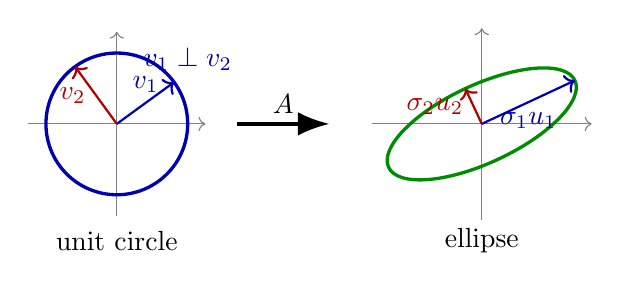
\begin{tikzpicture}[scale=0.9]
  % input circle
  \draw[->,gray] (-3.3,0) -- (-0.8,0);
  \draw[->,gray] (-2.05,-1.3) -- (-2.05,1.3);
  \draw[blue!70!black,very thick] (-2.05,0) circle (1);
  \draw[blue!70!black,thick,->] (-2.05,0) -- (-1.24,0.59)
    node[midway,above] {$v_1$};
  \draw[red!70!black,thick,->] (-2.05,0) -- (-2.64,0.81)
    node[midway,left] {$v_2$};
  \node[blue!70!black] at (-1.05,0.92) {$v_1\perp v_2$};
  \node at (-2.05,-1.65) {unit circle};

  % arrow
  \draw[-{Latex[length=4mm]},very thick] (-0.35,0) -- (0.95,0)
    node[midway,above] {$A$};

  % output ellipse
  \draw[->,gray] (1.55,0) -- (4.65,0);
  \draw[->,gray] (3.1,-1.35) -- (3.1,1.35);
  \begin{scope}[shift={(3.1,0)},rotate=25]
    \draw[green!55!black,very thick] (0,0) ellipse (1.45 and 0.55);
    \draw[blue!70!black,thick,->] (0,0) -- (1.45,0)
      node[midway,below] {$\sigma_1u_1$};
    \draw[red!70!black,thick,->] (0,0) -- (0,0.55)
      node[midway,left] {$\sigma_2u_2$};
  \end{scope}
  \node at (3.1,-1.65) {ellipse};
\end{tikzpicture}
\end{center}

\vspace{0.2cm}

\begin{center}
\x{The image of a round object has special axes.}
\end{center}

\end{frame}



\begin{frame}[shrink=10]{Contract First}

\[
\scriptsize
\boxed{
A
=
\underbrace{\Ucols}_{\substack{U\\\text{columns define }u_i}}
\underbrace{\Sigdisplay}_{\substack{\Sigma\\\text{diagonal entries define }\sigma_i}}
\underbrace{\Vrows}_{\substack{V^T\\\text{rows define }v_i^T}}
}.
\]

\vfill

\[
\scriptsize
\underbrace{\Vcols}_{V}
\qquad
\underbrace{\Vrows}_{V^T}
\qquad
\underbrace{\Vrows\Vcols=I}_{V^TV=I}.
\]

\end{frame}


\begin{frame}[shrink=18]{Contract Gives the Axis Equation}

\[
\tiny
\begin{aligned}
A
\underbrace{\Vcols}_{V}
&=
\left(
\underbrace{\Ucols}_{U}
\underbrace{\Sigdisplay}_{\Sigma}
\underbrace{\Vrows}_{V^T}
\right)
\underbrace{\Vcols}_{V}\\[0.5em]
&=
\underbrace{\Ucols}_{U}
\underbrace{\Sigdisplay}_{\Sigma}
\underbrace{\Vrows\Vcols}_{I}\\[0.5em]
&=
\underbrace{\Ucols}_{U}
\underbrace{\Sigdisplay}_{\Sigma}.
\end{aligned}
\]

\vfill

\[
\boxed{A\,V=U\Sigma.}
\]

\end{frame}


\begin{frame}[shrink=10]{Expand $AV$}

\[
\scriptsize
A
\underbrace{
\begin{pmatrix}
|&|& &|\\
\bl{v_1}&\rd{v_2}&\cdots&\gry{v_n}\\
|&|& &|
\end{pmatrix}}_{\substack{\text{special input directions}\\ V}}
=
\underbrace{
\begin{pmatrix}
|&|& &|\\
\bl{Av_1}&\rd{Av_2}&\cdots&\gry{Av_n}\\
|&|& &|
\end{pmatrix}}_{\text{left side columns}}.
\]

\end{frame}


\begin{frame}[shrink=10]{Expand $U\Sigma$}

\[
\scriptsize
\underbrace{
\begin{pmatrix}
|&|& &|\\
\bl{u_1}&\rd{u_2}&\cdots&\gry{u_n}\\
|&|& &|
\end{pmatrix}}_{\substack{U\\\text{output directions}}}
\underbrace{
\begin{pmatrix}
\bl{\sigma_1}&0&\cdots&0\\
0&\rd{\sigma_2}&\cdots&0\\
\vdots&\vdots&\ddots&\vdots\\
0&0&\cdots&\gry{0}
\end{pmatrix}}_{\substack{\Sigma\\\text{diagonal stretches}}}
=
\underbrace{
\begin{pmatrix}
|&|& &|\\
\bl{\sigma_1u_1}&\rd{\sigma_2u_2}&\cdots&\gry{0u_n}\\
|&|& &|
\end{pmatrix}}_{\text{right side columns}}.
\]

\end{frame}


\begin{frame}[shrink=8]{Compare Columns}

\[
\scriptsize
\underbrace{
\begin{pmatrix}
|&|& &|\\
\bl{Av_1}&\rd{Av_2}&\cdots&\gry{Av_n}\\
|&|& &|
\end{pmatrix}}_{AV}
=
\underbrace{
\begin{pmatrix}
|&|& &|\\
\bl{\sigma_1u_1}&\rd{\sigma_2u_2}&\cdots&\gry{0u_n}\\
|&|& &|
\end{pmatrix}}_{U\Sigma}.
\]

\vfill

\[
\scriptsize
\underbrace{\bl{Av_1=\sigma_1u_1}}_{\text{first column}},
\qquad
\underbrace{\rd{Av_2=\sigma_2u_2}}_{\text{second column}},
\qquad
\cdots,
\qquad
\underbrace{\gry{Av_n=0u_n}}_{\text{last zero column}}.
\]

\vfill

\[
\boxed{Av_i=\sigma_i u_i\quad\text{for every displayed column }i.}
\]

\end{frame}


\begin{frame}[shrink=8]{Notation: Singular Values}

\[
\scriptsize
\underbrace{\Sigdisplay}_{\substack{\Sigma\\\text{rectangular diagonal matrix}}}
\qquad
\underbrace{\bl{\sigma_1}\ge \rd{\sigma_2}\ge\cdots\ge \gry{0}}_{\text{axis lengths}}
\]

\vfill

\begin{center}
\x{The diagonal entries are the singular values; they are lengths, so they are nonnegative.}
\end{center}

\end{frame}


\begin{frame}[shrink=18]{What We Must Find}

\[
\scriptsize
\boxed{
A
=
\underbrace{\Ucols}_{\substack{U\\\text{output directions}}}
\underbrace{\Sigdisplay}_{\substack{\Sigma\\\text{nonnegative lengths}}}
\underbrace{\Vrows}_{\substack{V^T\\\text{input-coordinate rows}}}
}
\]

\vfill

\[
\scriptsize
\begin{aligned}
\underbrace{
A\Vcols
}_{\text{contract multiplied by }V}
&=
\underbrace{
\begin{pmatrix}|&|& &|\\
\bl{u_1}&\rd{u_2}&\cdots&\gry{u_n}\\
|&|& &|
\end{pmatrix}}_{U}
\underbrace{
\begin{pmatrix}
\bl{\sigma_1}&0&\cdots&0\\
0&\rd{\sigma_2}&\cdots&0\\
\vdots&\vdots&\ddots&\vdots\\
0&0&\cdots&\gry{0}
\end{pmatrix}}_{\Sigma}\\
\underbrace{
\begin{pmatrix}|&|& &|\\
\bl{Av_1}&\rd{Av_2}&\cdots&\gry{Av_n}\\
|&|& &|
\end{pmatrix}}_{\text{expanded left side}}
&=
\underbrace{
\begin{pmatrix}|&|& &|\\
\bl{\sigma_1u_1}&\rd{\sigma_2u_2}&\cdots&\gry{0u_n}\\
|&|& &|
\end{pmatrix}}_{\text{expanded right side}}.
\end{aligned}
\]

\vfill

\begin{center}
\x{Find the columns and the lengths; then the whole matrix is determined.}
\end{center}

\end{frame}



\begin{frame}[shrink=12]{Stack the Axis Equations}

\[
\scriptsize
\underbrace{
\begin{pmatrix}
|&|& &|\\
\bl{Av_1}&\rd{Av_2}&\cdots&\gry{Av_n}\\
|&|& &|
\end{pmatrix}}_{\displaystyle AV}
=
\underbrace{
\begin{pmatrix}
|&|& &|\\
\bl{\sigma_1u_1}&\rd{\sigma_2u_2}&\cdots&\gry{0u_n}\\
|&|& &|
\end{pmatrix}}_{\displaystyle U\Sigma}.
\]

\vfill

\[
\scriptsize
\underbrace{A\Vcols}_{AV}
=
\underbrace{\Ucols\Sigdisplay}_{U\Sigma}.
\]

\end{frame}


\begin{frame}[shrink=20]{From Axis Equations to SVD}

\[
\scriptsize
\underbrace{\Vrows}_{V^T}
\underbrace{\Vcols}_{V}
=I,
\qquad
\underbrace{V^{-1}=V^T}_{\text{orthogonal inverse}}.
\]

\vfill

\[
\scriptsize
A\underbrace{\Vcols}_{V}
=
\underbrace{\Ucols}_{U}
\underbrace{\Sigdisplay}_{\Sigma},
\]

\[
\scriptsize
A
\underbrace{\Vcols}_{V}
\underbrace{\Vrows}_{V^T}
=
\underbrace{\Ucols}_{U}
\underbrace{\Sigdisplay}_{\Sigma}
\underbrace{\Vrows}_{V^T}.
\]

\[
\scriptsize
\boxed{
A=
\svdproduct
}.
\]

\end{frame}


% ═══════════════════════════════════════
% §4 OUTPUT AXES AND THE THEOREM
% ADR: Continue from input axes. Students must see that v_i live on the
% input circle, while u_i are built after applying A. The proof follows
% real inner products only.
% ═══════════════════════════════════════
\section{Output Axes}

\begin{frame}[shrink=8]{Now Build the Output Axes}

\[
\scriptsize
\underbrace{A^TA}_{\text{input-side square}}
=
\underbrace{\Vcols}_{\substack{V\\\text{input axes }v_i}}
\underbrace{\SigTsigdisplay}_{\substack{\Sigma^T\Sigma\\\text{squared lengths }\sigma_i^2}}
\underbrace{\Vrows}_{V^T},
\]

\[
\scriptsize
\underbrace{A^TA v_i=\sigma_i^2v_i}_{\text{one input-axis column}}
\qquad
\underbrace{
\|Av_i\|^2
=v_i^TA^TAv_i
=\sigma_i^2v_i^Tv_i
=\sigma_i^2
}_{\text{output length computation}}.
\]

\vfill

\[
\scriptsize
\boxed{
\underbrace{u_i}_{\text{output axis direction}}
=
\underbrace{\frac{Av_i}{\sigma_i}}_{\text{normalized output vector}}
}
\qquad
\underbrace{\sigma_i>0}_{\text{nonzero axis}}.
\]

\vfill

\[
\scriptsize
\boxed{
\underbrace{Av_i}_{\text{actual output}}
=
\underbrace{\sigma_i u_i}_{\text{length times direction}}
}
\]

\end{frame}


\begin{frame}[fragile]{Input Axis Lands on Output Axis}

\begin{center}
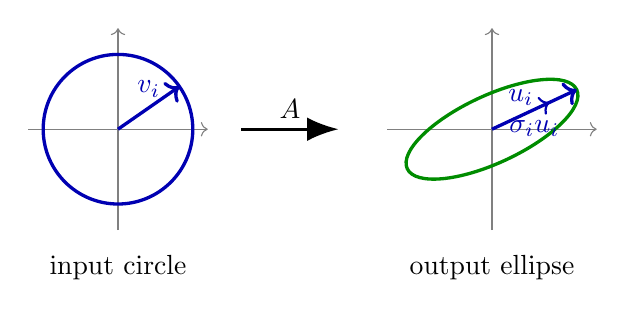
\begin{tikzpicture}[scale=0.95]
  % input circle
  \draw[->,gray] (-3.2,0)--(-0.8,0);
  \draw[->,gray] (-2,-1.35)--(-2,1.35);
  \draw[blue!70!black,very thick] (-2,0) circle (1);
  \draw[blue!70!black,->,very thick] (-2,0)--(-1.18,0.57) node[midway,above] {$v_i$};
  \node[below] at (-2,-1.55) {input circle};

  \draw[-{Latex[length=4mm]},very thick] (-0.35,0)--(0.95,0) node[midway,above] {$A$};

  % output ellipse
  \draw[->,gray] (1.6,0)--(4.4,0);
  \draw[->,gray] (3,-1.35)--(3,1.35);
  \begin{scope}[shift={(3,0)},rotate=25]
    \draw[green!55!black,very thick] (0,0) ellipse (1.25 and 0.45);
    \draw[blue!70!black,->,very thick] (0,0)--(1.25,0) node[midway,below] {$\sigma_i u_i$};
    \draw[blue!70!black,dashed,->,thick] (0,0)--(0.85,0) node[midway,above] {$u_i$};
  \end{scope}
  \node[below] at (3,-1.55) {output ellipse};
\end{tikzpicture}
\end{center}

\vspace{0.2cm}

\begin{center}
\x{$v_i$ is an input direction.  $u_i$ is the normalized output direction.}
\end{center}

\end{frame}


\begin{frame}{Check $u_i$ Has Length $1$}

$$
\underbrace{u_i}_{\text{output unit direction}}
=
\underbrace{\frac{Av_i}{\sigma_i}}_{\text{normalize the output vector}}.
$$

\vfill

\[
\scriptsize
\|u_i\|
=\left\|\frac{Av_i}{\sigma_i}\right\|
=\frac{\|Av_i\|}{\sigma_i}
=\frac{\sigma_i}{\sigma_i}
=1.
\]

\vfill

\begin{center}
\x{Each nonzero output axis direction is a unit vector.}
\end{center}

\end{frame}


\begin{frame}[shrink=8]{Why Different Output Axes Are Orthogonal}

\[
\scriptsize
\underbrace{i\ne j}_{\text{different axes}}
\qquad\Longrightarrow\qquad
\underbrace{u_i^Tu_j}_{\text{test orthogonality}}
=\frac{(Av_i)^T(Av_j)}{\sigma_i\sigma_j}.
\]

\vfill

\[
\scriptsize
u_i^Tu_j
=\frac{v_i^TA^TAv_j}{\sigma_i\sigma_j}.
\]

\vfill

\[
\scriptsize
u_i^Tu_j
=\frac{\sigma_j^2}{\sigma_i\sigma_j}v_i^Tv_j
=0.
\]

\end{frame}


\begin{frame}{Inner-Product Table}

\vfill

\begin{center}
\renewcommand{\arraystretch}{1.5}
\begin{tabular}{c|ccc}
 & $\bl{u_1}$ & $\rd{u_2}$ & $\gry{u_3}$\\
\hline
$\bl{u_1^T}$ & $\bl{1}$ & $0$ & $0$\\
$\rd{u_2^T}$ & $0$ & $\rd{1}$ & $0$\\
$\gry{u_3^T}$ & $0$ & $0$ & $\gry{1}$
\end{tabular}
\end{center}

\vfill

\[
\scriptsize
\underbrace{\Urows}_{U^T}
\underbrace{\Ucols}_{U}
=
\underbrace{
\begin{pmatrix}
1&0&0\\
0&1&0\\
0&0&1
\end{pmatrix}}_{\text{inner-product table}}.
\]

\end{frame}


\begin{frame}[shrink=8]{What If $\sigma_i=0$?}

\[
\scriptsize
\underbrace{\sigma_i=0}_{\text{zero singular value}}
\qquad\Longrightarrow\qquad
\underbrace{A^TA v_i=0}_{\text{eigenvalue }0}.
\]

\vfill

\[
\scriptsize
\underbrace{\|Av_i\|^2}_{\text{squared output length}}
=
\underbrace{(Av_i)^T(Av_i)}_{\text{definition of length}}
=
\underbrace{v_i^TA^TA v_i}_{\text{move }A\text{ to the middle}}
=
\underbrace{v_i^T0}_{A^TA v_i=0}
=0.
\]

\vfill

\[
\boxed{\underbrace{Av_i=0}_{\text{invisible input direction}}.}
\]

\vfill

\begin{center}
\x{Zero singular value = invisible input direction.}
\end{center}

\end{frame}


\begin{frame}[fragile]{Visible and Invisible Directions}

\begin{center}
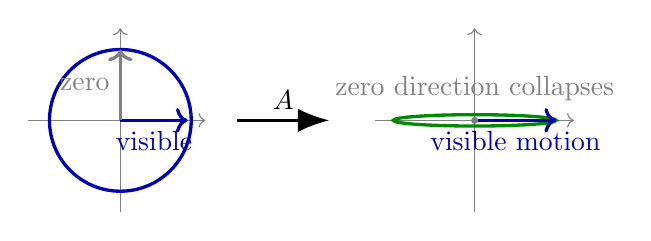
\begin{tikzpicture}[scale=0.9]
  \draw[->,gray] (-3.3,0)--(-0.8,0);
  \draw[->,gray] (-2,-1.3)--(-2,1.3);
  \draw[blue!70!black,very thick] (-2,0) circle (1);
  \draw[blue!70!black,->,very thick] (-2,0)--(-1.05,0) node[midway,below] {visible};
  \draw[gray,->,very thick] (-2,0)--(-2,1) node[midway,left] {zero};

  \draw[-{Latex[length=4mm]},very thick] (-0.35,0)--(0.95,0) node[midway,above] {$A$};

  \draw[->,gray] (1.6,0)--(4.4,0);
  \draw[->,gray] (3,-1.3)--(3,1.3);
  \draw[green!55!black,very thick] (3,0) ellipse (1.15 and 0.08);
  \draw[blue!70!black,->,very thick] (3,0)--(4.15,0) node[midway,below] {visible motion};
  \fill[gray] (3,0) circle (0.05);
  \node[gray] at (3,0.45) {zero direction collapses};
\end{tikzpicture}
\end{center}

\vspace{0.25cm}

\begin{center}
\x{The null space is exactly the collection of invisible directions.}
\end{center}

\end{frame}


\begin{frame}{Complete the Output Basis}

$$
\underbrace{u_1,\ldots,u_r}_{\text{directions from nonzero singular values}}
\quad\leadsto\quad
\underbrace{u_1,\ldots,u_r,u_{r+1},\ldots,u_m}_{\text{full output orthonormal basis}}.
$$

\vfill

$$
\underbrace{\operatorname{Col}(A)^\perp}_{\text{missing output directions}}
=
\underbrace{\operatorname{Null}(A^T)}_{\text{projection-complement source}}.
$$

\vfill

\begin{center}
\x{This gives a full orthogonal matrix $U$.}
\end{center}

\end{frame}


\begin{frame}{Callback: Complete by Projection Complement}

$$
B=
\underbrace{\begin{pmatrix}
|&|&&|\\
u_1&u_2&\cdots&u_r\\
|&|&&|
\end{pmatrix}}_{\text{existing output axes}}.
$$

\vfill

$$
\underbrace{P}_{\text{projection onto known axes}}
=
\underbrace{BB^T}_{\text{diagonal cross-fill of known columns}}.
$$

\vfill

$$
\underbrace{I-P}_{\text{orthogonal complement projection}}.
$$

\begin{center}
\x{This is exactly the previous projection-complement method.}
\end{center}

\end{frame}


\begin{frame}{Diagonal Cross-Fill the Complement}

\vfill

$$
\underbrace{I-P}_{\text{complement projection}}
=
\underbrace{w_{r+1}w_{r+1}^T+\cdots+w_mw_m^T}_{\text{rank-one orthogonal projections}}.
$$

\vfill

\begin{center}
\x{Now the missing directions come from the same old machine.}
\end{center}

\end{frame}


\begin{frame}{Complement Gives Missing Axes}

$$
\underbrace{I-P}_{\text{complement projection}}
=
\underbrace{w_{r+1}w_{r+1}^T+\cdots+w_mw_m^T}_{\text{diagonal cross-fill output}}.
$$

\vfill

$$
\underbrace{u_{r+1},\ldots,u_m}_{\text{missing output axes}}
=
\underbrace{w_{r+1},\ldots,w_m}_{\text{orthonormal complement vectors}}.
$$

\end{frame}


\begin{frame}[shrink=12]{Stack Everything}

$$
\underbrace{Av_i}_{\text{output from input axis}}
=
\underbrace{\sigma_i u_i}_{\text{axis length times output direction}}.
$$

\vfill

\[
\scriptsize
\underbrace{
\begin{pmatrix}
|&|& &|\\
\bl{Av_1}&\rd{Av_2}&\cdots&\gry{Av_n}\\
|&|& &|
\end{pmatrix}}_{AV}
=
\underbrace{
\begin{pmatrix}
|&|& &|\\
\bl{\sigma_1u_1}&\rd{\sigma_2u_2}&\cdots&\gry{0u_n}\\
|&|& &|
\end{pmatrix}}_{U\Sigma}.
\]

\[
\scriptsize
\boxed{
A\underbrace{\Vcols}_{V}
=
\underbrace{\Ucols}_{U}
\underbrace{\Sigdisplay}_{\Sigma}
}.
\]

\end{frame}


\begin{frame}[shrink=20]{Singular Value Decomposition}

$$
\underbrace{\Vrows}_{V^T}
\underbrace{\Vcols}_{V}
=I,
\qquad
\underbrace{V^{-1}=V^T}_{\text{orthogonal inverse}}.
$$

\vfill

\[
\scriptsize
\underbrace{
\begin{pmatrix}
|&|& &|\\
\bl{Av_1}&\rd{Av_2}&\cdots&\gry{Av_n}\\
|&|& &|
\end{pmatrix}}_{AV}
=
\underbrace{
\begin{pmatrix}
|&|& &|\\
\bl{\sigma_1u_1}&\rd{\sigma_2u_2}&\cdots&\gry{0u_n}\\
|&|& &|
\end{pmatrix}}_{U\Sigma},
\]

\[
\scriptsize
A
\underbrace{\Vcols}_{V}
\underbrace{\Vrows}_{V^T}
=
\underbrace{\Ucols}_{U}
\underbrace{\Sigdisplay}_{\Sigma}
\underbrace{\Vrows}_{V^T}.
\]

\[
\scriptsize
\boxed{
A=
\underbrace{\Ucols}_{U}
\underbrace{\Sigdisplay}_{\Sigma}
\underbrace{\Vrows}_{V^T}
}.
\]

\end{frame}


\begin{frame}[shrink=20]{Theorem}

\[
\scriptsize
\boxed{
A=
\underbrace{\Ucols}_{\substack{U\\\text{orthogonal output matrix}}}
\underbrace{\Sigdisplay}_{\substack{\Sigma\\\text{nonnegative rectangular diagonal}}}
\underbrace{\Vrows}_{\substack{V^T\\\text{orthogonal input coordinates}}}
}.
\]

\vfill

\begin{thm}[Singular Value Decomposition]
For every real $m\times n$ matrix $A$, there exist orthogonal matrices
$U$ and $V$, and a rectangular diagonal matrix $\Sigma$ with nonnegative
entries, such that the displayed factorization holds.
\end{thm}

\vfill

\begin{center}
\x{Every real matrix maps balls to ellipsoids with orthogonal axes.}
\end{center}

\end{frame}


\begin{frame}[shrink=18]{Proof Photograph}

\[
\tiny
\begin{aligned}
\underbrace{A^TA}_{\text{real symmetric}}
&=
\underbrace{\Vcols}_{V}
\underbrace{\SigTsigdisplay}_{\Sigma^T\Sigma}
\underbrace{\Vrows}_{V^T}\\[0.4em]
\underbrace{A^TA v_i=\sigma_i^2v_i}_{\text{input eigen-axis}}
&\Longrightarrow
\underbrace{\|Av_i\|^2=v_i^TA^TAv_i=\sigma_i^2}_{\text{axis length}}\\[0.4em]
\underbrace{u_i=\dfrac{Av_i}{\sigma_i}}_{\text{normalize nonzero output}}
&\Longrightarrow
\underbrace{Av_i=\sigma_i u_i}_{\text{axis equation}}\\[0.4em]
\underbrace{
\begin{pmatrix}|&|& &|\\
\bl{Av_1}&\rd{Av_2}&\cdots&\gry{Av_n}\\
|&|& &|
\end{pmatrix}}_{AV}
&=
\underbrace{
\begin{pmatrix}|&|& &|\\
\bl{\sigma_1u_1}&\rd{\sigma_2u_2}&\cdots&\gry{0u_n}\\
|&|& &|
\end{pmatrix}}_{U\Sigma}\\[0.4em]
\underbrace{AV=U\Sigma}_{\text{stacked columns}}
&\Longrightarrow
\underbrace{
A=
\underbrace{\Ucols}_{U}
\underbrace{\Sigdisplay}_{\Sigma}
\underbrace{\Vrows}_{V^T}
}_{\text{right multiply by }V^T}.
\end{aligned}
\]

\vfill

\begin{center}
\x{The whole proof is real symmetric diagonalization of $A^TA$.}
\end{center}

\end{frame}



% ═══════════════════════════════════════
% §5 METHOD SUMMARY
% ADR: Stop at the decomposition method. Do not turn this into a
% statistics course. Applications can be saved for a future module.
% ═══════════════════════════════════════
\section{Method Summary}

\begin{frame}[shrink=18]{The Method}

\[
\tiny
\underbrace{A^TA}_{\text{real symmetric matrix to compute}}
=
\underbrace{\Vcols}_{V}
\underbrace{\SigTsigdisplay}_{\Sigma^2}
\underbrace{\Vrows}_{V^T}.
\]

\vfill

\[
\tiny
\underbrace{u_i=\frac{Av_i}{\sigma_i}}_{\substack{\text{define output axis}\\\sigma_i>0}}
\qquad
\underbrace{
B=
\begin{pmatrix}|&|& &|\\
u_1&u_2&\cdots&u_r\\
|&|& &|
\end{pmatrix}}_{\text{known output axes}}
\qquad
\underbrace{P=BB^T}_{\text{known-axis projection}}
\qquad
\underbrace{I-P}_{\text{missing-axis projection}}.
\]

\vfill

\[
\tiny
\begin{aligned}
\underbrace{
\begin{pmatrix}|&|& &|\\
\bl{Av_1}&\rd{Av_2}&\cdots&\gry{Av_n}\\
|&|& &|
\end{pmatrix}}_{AV}
&=
\underbrace{
\begin{pmatrix}|&|& &|\\
\bl{\sigma_1u_1}&\rd{\sigma_2u_2}&\cdots&\gry{0u_n}\\
|&|& &|
\end{pmatrix}}_{U\Sigma}\\[0.4em]
\underbrace{A\Vcols=U\Sigma}_{\text{stacked axis equations}}
&\Longrightarrow
\underbrace{A=
\underbrace{\Ucols}_{U}
\underbrace{\Sigdisplay}_{\Sigma}
\underbrace{\Vrows}_{V^T}}_{\text{SVD contract}}.
\end{aligned}
\]

\end{frame}


% ═══════════════════════════════════════
% §6 WORKED EXERCISE
% ADR: The exercise must be a complete auditable computation. Every object
% appears entrywise/columnwise before the concept name is used.
% ═══════════════════════════════════════
\section{Worked Exercise}

\begin{frame}[shrink=10]{Exercise: Start With a $3\times2$ Matrix}

\[
\scriptsize
\underbrace{
A=
\begin{pmatrix}
1&1\\
1&1\\
0&0
\end{pmatrix}}_{\substack{\text{two input coordinates}\\\text{three output coordinates}}}
\qquad
\underbrace{
A^T=
\begin{pmatrix}
1&1&0\\
1&1&0
\end{pmatrix}}_{\text{rowwise transpose}}.
\]

\vfill

\[
\scriptsize
\underbrace{
\begin{pmatrix}
1&1&0\\
1&1&0
\end{pmatrix}}_{A^T}
\underbrace{
\begin{pmatrix}
1&1\\
1&1\\
0&0
\end{pmatrix}}_{A}
=
\underbrace{
\begin{pmatrix}
2&2\\
2&2
\end{pmatrix}}_{A^TA}.
\]

\vfill

\begin{center}
\x{The input-side square matrix is only $2\times2$.}
\end{center}

\end{frame}


\begin{frame}[shrink=10]{Spectral Projections of $A^TA$}

\[
\scriptsize
\underbrace{
\begin{pmatrix}
2&2\\
2&2
\end{pmatrix}}_{B=A^TA}
=
\underbrace{
\bl{4}P_{\bl{4}}+\rd{0}P_{\rd{0}}}_{\text{spectral decomposition form}},
\qquad
\underbrace{\lambda_1=\bl{4},\ \lambda_2=\rd{0}}_{\det(tI-B)=t(t-4)}.
\]

\vfill

\[
\scriptsize
\underbrace{P_{\bl{4}}}_{\text{spectral projection for }\lambda=4}
=
\underbrace{\frac{B-0I}{4-0}}_{\text{Lagrange projection polynomial}}
=
\underbrace{\frac14
\begin{pmatrix}
2&2\\
2&2
\end{pmatrix}}_{\frac14B}
=
\underbrace{
\begin{pmatrix}
\frac12&\frac12\\
\frac12&\frac12
\end{pmatrix}}_{P_{\bl{4}}}.
\]

\vfill

\[
\scriptsize
\underbrace{P_{\rd{0}}}_{\text{spectral projection for }\lambda=0}
=
\underbrace{\frac{B-4I}{0-4}}_{\text{Lagrange projection polynomial}}
=
\underbrace{
\begin{pmatrix}
\frac12&-\frac12\\
-\frac12&\frac12
\end{pmatrix}}_{P_{\rd{0}}}.
\]

\end{frame}


\begin{frame}[shrink=10]{Diagonal Cross-Fill the Projections}

\[
\scriptsize
\underbrace{
\begin{pmatrix}
\frac12&\frac12\\
\frac12&\frac12
\end{pmatrix}}_{P_{\bl{4}}}
=
\underbrace{
\begin{pmatrix}
\frac1{\sqrt2}\\[0.15em]
\frac1{\sqrt2}
\end{pmatrix}
\begin{pmatrix}
\frac1{\sqrt2}&\frac1{\sqrt2}
\end{pmatrix}}_{\bl{v_1v_1^T}}.
\]

\vfill

\[
\scriptsize
\underbrace{
\begin{pmatrix}
\frac12&-\frac12\\
-\frac12&\frac12
\end{pmatrix}}_{P_{\rd{0}}}
=
\underbrace{
\begin{pmatrix}
\frac1{\sqrt2}\\[0.15em]
-\frac1{\sqrt2}
\end{pmatrix}
\begin{pmatrix}
\frac1{\sqrt2}&-\frac1{\sqrt2}
\end{pmatrix}}_{\rd{v_2v_2^T}}.
\]

\vfill

\[
\scriptsize
\underbrace{\bl{v_1}=
\begin{pmatrix}
\frac1{\sqrt2}\\[0.15em]
\frac1{\sqrt2}
\end{pmatrix}}_{\text{cross-filled from }P_{\bl{4}}}
\qquad
\underbrace{\rd{v_2}=
\begin{pmatrix}
\frac1{\sqrt2}\\[0.15em]
-\frac1{\sqrt2}
\end{pmatrix}}_{\text{cross-filled from }P_{\rd{0}}}.
\]

\end{frame}


\begin{frame}[shrink=10]{Input Axes and Squared Singular Values}

\[
\scriptsize
\underbrace{
\begin{pmatrix}
|&|\\
\bl{v_1}&\rd{v_2}\\
|&|
\end{pmatrix}}_{V}
=
\underbrace{
\begin{pmatrix}
\frac1{\sqrt2}&\frac1{\sqrt2}\\[0.15em]
\frac1{\sqrt2}&-\frac1{\sqrt2}
\end{pmatrix}}_{\text{orthogonal input axes}},
\qquad
\underbrace{
\begin{pmatrix}
\bl{4}&0\\
0&\rd{0}
\end{pmatrix}}_{\Sigma^T\Sigma}.
\]

\end{frame}


\begin{frame}[shrink=12]{Apply $A$ to the Input Axes}

\[
\scriptsize
\underbrace{
\begin{pmatrix}
1&1\\
1&1\\
0&0
\end{pmatrix}}_{A}
\underbrace{
\begin{pmatrix}
\frac1{\sqrt2}\\[0.15em]
\frac1{\sqrt2}
\end{pmatrix}}_{\bl{v_1}}
=
\underbrace{
\begin{pmatrix}
\sqrt2\\
\sqrt2\\
0
\end{pmatrix}}_{\bl{Av_1}}
=
\underbrace{2}_{\bl{\sigma_1}}
\underbrace{
\begin{pmatrix}
\frac1{\sqrt2}\\[0.15em]
\frac1{\sqrt2}\\[0.15em]
0
\end{pmatrix}}_{\bl{u_1}}.
\]

\vfill

\[
\scriptsize
\underbrace{
\begin{pmatrix}
1&1\\
1&1\\
0&0
\end{pmatrix}}_{A}
\underbrace{
\begin{pmatrix}
\frac1{\sqrt2}\\[0.15em]
-\frac1{\sqrt2}
\end{pmatrix}}_{\rd{v_2}}
=
\underbrace{
\begin{pmatrix}
0\\
0\\
0
\end{pmatrix}}_{\rd{Av_2}}
=
\underbrace{0}_{\rd{\sigma_2}}
\underbrace{\rd{u_2}}_{\text{not fixed by }Av_2}.
\]

\end{frame}


\begin{frame}[shrink=10]{Projection Onto the Known Output Axis}

\[
\scriptsize
\underbrace{
B=
\begin{pmatrix}
|\\
\bl{u_1}\\
|
\end{pmatrix}
=
\begin{pmatrix}
\frac1{\sqrt2}\\[0.15em]
\frac1{\sqrt2}\\[0.15em]
0
\end{pmatrix}}_{\text{known output-axis matrix}}
\]

\vfill

\[
\scriptsize
\underbrace{P}_{\text{projection onto known output axis}}
=
\underbrace{BB^T}_{\text{diagonal cross-fill}}
=
\underbrace{
\begin{pmatrix}
\frac1{\sqrt2}\\[0.15em]
\frac1{\sqrt2}\\[0.15em]
0
\end{pmatrix}
\begin{pmatrix}
\frac1{\sqrt2}&\frac1{\sqrt2}&0
\end{pmatrix}}_{\bl{u_1u_1^T}}
=
\underbrace{
\begin{pmatrix}
\frac12&\frac12&0\\
\frac12&\frac12&0\\
0&0&0
\end{pmatrix}}_{P}.
\]

\end{frame}


\begin{frame}[shrink=10]{Cross-Fill the Complement $I-P$}

\[
\scriptsize
\underbrace{I-P}_{\text{missing-output projection}}
=
\underbrace{
\begin{pmatrix}
\frac12&-\frac12&0\\
-\frac12&\frac12&0\\
0&0&1
\end{pmatrix}}_{\text{entrywise complement}}.
\]

\vfill

\[
\scriptsize
\underbrace{I-P}_{\text{complement projection}}
=
\underbrace{
\begin{pmatrix}
\frac1{\sqrt2}\\[0.15em]
-\frac1{\sqrt2}\\[0.15em]
0
\end{pmatrix}
\begin{pmatrix}
\frac1{\sqrt2}&-\frac1{\sqrt2}&0
\end{pmatrix}}_{\rd{u_2u_2^T}}
+
\underbrace{
\begin{pmatrix}
0\\0\\1
\end{pmatrix}
\begin{pmatrix}
0&0&1
\end{pmatrix}}_{\gry{u_3u_3^T}}.
\]

\vfill

\[
\scriptsize
\underbrace{\rd{u_2}=
\begin{pmatrix}
\frac1{\sqrt2}\\[0.15em]
-\frac1{\sqrt2}\\[0.15em]
0
\end{pmatrix}}_{\text{missing output axis}}
\qquad
\underbrace{\gry{u_3}=
\begin{pmatrix}
0\\0\\1
\end{pmatrix}}_{\text{extra output axis}}.
\]

\end{frame}


\begin{frame}[shrink=8]{Stack the Exercise Columns}

\[
\scriptsize
\underbrace{
A
\begin{pmatrix}
|&|\\
\bl{v_1}&\rd{v_2}\\
|&|
\end{pmatrix}}_{AV}
=
\underbrace{
\begin{pmatrix}
|&|\\
\bl{Av_1}&\rd{Av_2}\\
|&|
\end{pmatrix}}_{\text{computed outputs}}
=
\underbrace{
\begin{pmatrix}
|&|\\
\bl{2u_1}&\rd{0u_2}\\
|&|
\end{pmatrix}}_{\text{stretched output axes}}.
\]

\vfill

\[
\scriptsize
\underbrace{
\begin{pmatrix}
|&|&|\\
\bl{u_1}&\rd{u_2}&\gry{u_3}\\
|&|&|
\end{pmatrix}}_{U}
\underbrace{
\begin{pmatrix}
\bl{2}&0\\
0&\rd{0}\\
0&0
\end{pmatrix}}_{\Sigma}
=
\underbrace{
\begin{pmatrix}
|&|\\
\bl{2u_1}&\rd{0u_2}\\
|&|
\end{pmatrix}}_{U\Sigma}.
\]

\end{frame}


\begin{frame}[shrink=18]{Exercise Answer}

\[
\scriptsize
\underbrace{
U=
\begin{pmatrix}
\frac1{\sqrt2}&\frac1{\sqrt2}&0\\[0.15em]
\frac1{\sqrt2}&-\frac1{\sqrt2}&0\\[0.15em]
0&0&1
\end{pmatrix}}_{\text{output orthogonal matrix}}
\qquad
\underbrace{
\Sigma=
\begin{pmatrix}
2&0\\
0&0\\
0&0
\end{pmatrix}}_{\text{rectangular diagonal}}
\qquad
\underbrace{
V^T=
\begin{pmatrix}
\frac1{\sqrt2}&\frac1{\sqrt2}\\[0.15em]
\frac1{\sqrt2}&-\frac1{\sqrt2}
\end{pmatrix}}_{\text{input-coordinate rows}}.
\]

\vfill

\[
\tiny
\boxed{
\underbrace{
\begin{pmatrix}
1&1\\
1&1\\
0&0
\end{pmatrix}}_{A}
=
\underbrace{
\begin{pmatrix}
\frac1{\sqrt2}&\frac1{\sqrt2}&0\\[0.15em]
\frac1{\sqrt2}&-\frac1{\sqrt2}&0\\[0.15em]
0&0&1
\end{pmatrix}}_{U}
\underbrace{
\begin{pmatrix}
2&0\\
0&0\\
0&0
\end{pmatrix}}_{\Sigma}
\underbrace{
\begin{pmatrix}
\frac1{\sqrt2}&\frac1{\sqrt2}\\[0.15em]
\frac1{\sqrt2}&-\frac1{\sqrt2}
\end{pmatrix}}_{V^T}
}.
\]

\end{frame}


\begin{frame}{What Each Piece Means}

\[
\scriptsize
\boxed{
A=
\underbrace{\Ucols}_{\substack{U\\\text{orthonormal output axes}}}
\underbrace{\Sigdisplay}_{\substack{\Sigma\\\text{axis lengths of output ellipsoid}}}
\underbrace{\Vrows}_{\substack{V^T\\\text{orthonormal input-axis coordinates}}}
}.
\]

\vfill

\begin{center}
\x{Input axes $\to$ stretch lengths $\to$ output axes.}
\end{center}

\end{frame}


\begin{frame}[shrink=15]{The Whole Story in One Line}

$$
\underbrace{Av_i}_{\text{image of input axis}}
=
\underbrace{\sigma_i u_i}_{\text{stretched output axis}}.
$$

\vfill

\[
\scriptsize
A
\underbrace{\Vcols}_{V}
=
\underbrace{\Ucols}_{U}
\underbrace{\Sigdisplay}_{\Sigma}.
\]

\[
\scriptsize
\boxed{
A=
\svdproduct
}.
\]

\end{frame}


\begin{frame}[shrink=15]{Final Summary}

$$
\boxed{
\underbrace{\text{round ball}}_{\text{all unit inputs}}
\xrightarrow{\ A\ }
\underbrace{\text{ellipsoid with orthogonal axes}}_{\text{visible output shape}}
}.
$$

\vfill

\[
\scriptsize
\boxed{
A=
\underbrace{\Ucols}_{\substack{U\\\text{output axes}}}
\underbrace{\Sigdisplay}_{\substack{\Sigma\\\text{axis lengths}}}
\underbrace{\Vrows}_{\substack{V^T\\\text{input-axis coordinates}}}
}.
\]

\vfill

\begin{center}
{\Large \x{SVD records exactly this geometry.}}
\end{center}

\end{frame}

\end{document}
